\documentclass[conference]{IEEEtran}
\IEEEoverridecommandlockouts
\usepackage{cite}
\usepackage{amsmath,amssymb,amsfonts}
\usepackage{flushend}
\usepackage{algorithm, algorithmic}
\usepackage{graphicx}
\usepackage{textcomp}
\usepackage{fancyhdr}
\pagestyle{fancy}
\def\BibTeX{{\rm B\kern-.05em{\sc i\kern-.025em b}\kern-.08em\kern-.1667em\lower.7ex\hbox{E}\kern-.125emX}}
\makeatletter
\newcommand*\titleheader[1]{\gdef\@titleheader{#1}}
\AtBeginDocument{%
  \let\st@red@title\@title
  \def\@title{%
    \vskip1.5em\st@red@title}
}
\makeatother
\title{Fault-Tolerant Application Specific\\ Network-on-Chip Design
\thanks{This work is partially supported by the research project No. ECR/2016/001389 dt. 06/03/2017, sponsored by the SERB, Govt. of India}
}
\fancyhf{}
\renewcommand{\headrulewidth}{0pt}
\cfoot{\textit{2017 Seventh International Symposium on Embedded Computing and System Design (ISED)}}
\IEEEoverridecommandlockouts\IEEEpubid{\makebox[\columnwidth]{978-1-5386-3032-7/17/\$31.00~\copyright~2017 IEEE \hfill} \hspace{\columnsep}\makebox[\columnwidth]{}}
\begin{document}
\author{\IEEEauthorblockN{Parth Shah\IEEEauthorrefmark{1},
Abhishek Kanniganti\IEEEauthorrefmark{2},
Soumya J\IEEEauthorrefmark{3}}
\IEEEauthorblockA{Department of Electrical and Electronics Engineering,\\
Birla Institute of Technology and Science - Pilani, Hyderabad Campus,\\
Hyderabad, India\\fo
Email: \IEEEauthorrefmark{1}parthjshah95@gmail.com,
\IEEEauthorrefmark{2}nmabhi42@gmail.com,
\IEEEauthorrefmark{3}soumyatkgp@gmail.com}}
\maketitle
\begin{abstract}
Network-on-Chip (NoC) has been introduced to address the communication problems associated with the traditional bus based System-on-Chip (SoC) architectures. NoC can be designed either using regular or irregular architectures. Even though many regular architectures have been proposed in the literature, there is a mismatch between the application requirements and the design. Application specific NoC designs have been proposed to match the requirements of the applications, which are irregular in nature. Due to the heavy integration of the components on the chip, designs that are vulnerable to faults in links can render the chip unusable. This paper first sets the benchmark of minimum possible communication cost and thereafter proposes a greedy algorithm to develop link fault-tolerant application specific topology for the given application core graph which meets that benchmark.
\end{abstract}
\begin{IEEEkeywords}
Link fault tolerance, greedy algorithm, application specific network on chip, topology design, graph theory
\end{IEEEkeywords}
\section{Introduction}
Recent advances in technology have enabled to integrate millions of transistors on a single chip, so much so that multiple components can now be integrated on a single chip, leading to the development of System-on-chip (SoC). Traditional SoC designs used bus topology for the communication between the components. But this can lead to saturation very fast and is not scalable. Network-on-Chip (NoC)\cite{b1} has been introduced to overcome the problems associated with bus based communication. For generic NoC, symmetric topologies like mesh are widely used, but there is a mismatch between the regular topologies and the application requirements. However, for Application Specific NoC (ASNoC), irregular topologies can reduce hardware costs and improve performance. A survey of ASNoC design techniques has been presented in\cite{b2, b3, b8}. They enumerate the advantages of custom topologies over standard ones for ASNoC. 

The network components which connect various cores in the NoC are prone to failure and can result in the complete breakdown of the system%[citation needed]
. Hence, it is essential to design NoC topologies with fault tolerance, which can be attained by adding more links and routers to the existing topology and create alternate paths between routers and cores. The proposed solution in this paper is a graph theoretic greedy algorithm that generates a link fault tolerant topology from the given application specifications with minimum communication cost.
\section{Related Work}
%the commented text in below paragraph will be included in the journal paper where we tackle router fault tolerance too.
A fault-tolerant irregular topology generation method has been presented in \cite{b3} for Application Specific NoC designs. They discuss how designed NoC topology allows different routing paths if there is a link failure on the default routing path. The solution proposed in this paper generates a fault tolerant topology by first generating random irregular non-fault tolerant topologies and adding additional links to make them fault tolerant. They compare fault-tolerant topologies with non-fault-tolerant application-specific irregular topologies on energy consumption, performance, and area using multimedia benchmarks and custom-generated graphs. They have used simulated annealing for the mapping process. However, %they have not considered the effect of faults on the routers or cores in the network. Also, %
the mapping has been considered after the topology is generated instead of considering the application requirements while synthesising the topology.

A fault-tolerant application-specific NoC architecture has been presented in\cite{b4} to tolerate permanent router failures. They have implemented the architecture in VHDL and synthesized in Xilinx ISE. They have proposed spare router and a link-interface in the network by considering 3-dimensional NoC and shown the results in 2-D environment as well. However, they have considered Through-Silicon-Vias (TSVs) in the process. To apply the same techniques to 2-D, the assumptions to be made must be different than that of 3-D, which has not been addressed.  The same group has presented a fault-tolerant application-specific NoC design in\cite{b5}. However, they have shown the simulation results only on mesh architectures instead of application-specific topology.

In\cite{b10} algorithms from three different domains for the construction of fault-tolerant graphs are evaluated. Classical graph-theoretic algorithms, optimization and bio-inspired approaches are compared regarding the quality of the generated graphs as well as concerning the runtime requirements.

Fault-tolerant application-specific NoC design has been implemented in\cite{b6} using FPGA. However, the implementation methods have not been given in detail and they have not explored the architectural optimizations while implementing on FPGA.

\cite{b11} demonstrates a fault tolerant topology where its dual-port network interface (NI) makes the key PE have two links with network at least, which can ensure high reliability of the system. An adaptive fault tolerant routing algorithm is also developed that can sense congestion on the network to work around the issues effectively.
 
 In\cite{b7}, they use the generalized binary de Bruijn's (GBDB) graph as a scalable and efficient network topology for an on-chip communication network. The experimental results show that the latency and energy consumption of generalized de Bruijn's graph are much less compared to Mesh and Torus, the two common NoC architectures in the literature. Hence, this paper compares the De Bruijn's topology with the one presented here.
\section{Problem Definition}
Input to our approach is an application which gives information such as the number of cores and the communication bandwidth requirement between each pair of cores. Our objective is to create topologies which have: \begin{enumerate}\item cores communicating with each other through at least two distinct paths,\item minimum latency and energy consumption and \item less hardware overheads.\end{enumerate}To achieve this, each link must be such that even if it is removed from the topology, the two routers which were connected would still be able to have connection using an alternate path. Thus, even if the link fails, the routers will not get cut off from each other. Also, latency and power consumption are assumed to be directly proportional to the total communication cost defined in section~\ref{commCostDef}.%needs citation
\begin{figure}
\centering
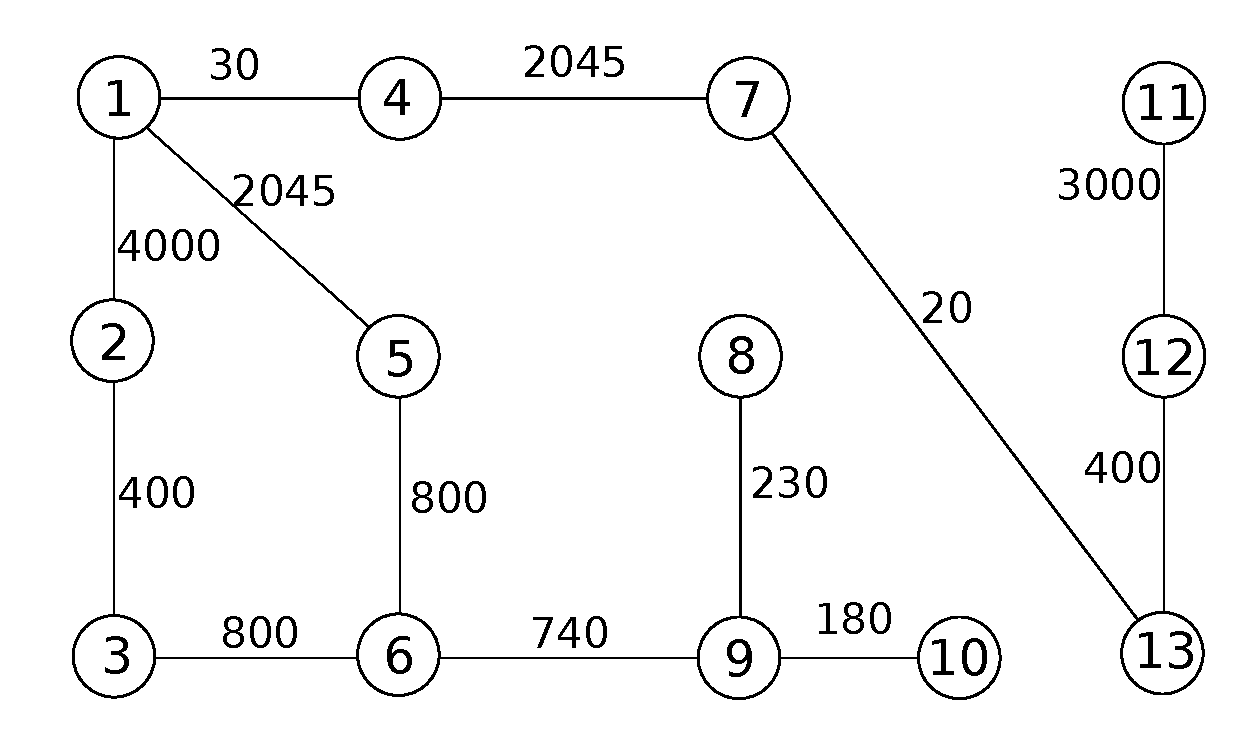
\includegraphics[width=0.35\textwidth]{../Figures_and_tables/Figure1_CoreFlowGraph}
\caption{Sample input core flow graph}
\label{inputFig}
\end{figure}
\subsection{Core Flow Graph and Topology Graph}
The application information is given with the help of a core flow graph (CFG) as defined in\cite{b3}:
\begin{quote}
A core flow graph (CFG) is a graph $G(N,E)$ where each vertex $n_i \in N$ represents a core (i.e., a node) in the application, and each edge $e_{i,j} \in E$ represents a dependency between two cores $n_i$ and $n_j$. The amount of data transfer between $n_i$ and $n_j$ is represented by the weight $w_{i,j}$ for all $e_{i,j}$ and is given in bits per second.
\end{quote}
A sample CFG is shown in fig.~\ref{inputFig}. The output is a network of routers or topology where each router is mapped to a core. This can be represented by the topology graph (TG) defined in\cite{b3}:
\begin{quote}
A topology graph (TG) is a connected graph $T(R,L)$ where $R$ represents the set of routers and $L$ represents the set of links connecting the routers.
\end{quote}
\subsection{Communication cost}\label{commCostDef}
In the CFG, for every edge $e_{i,j}$, the communication cost $c_{i,j}$ associated with it is the product of its weight $w_{i,j}$ and the number of hops from $r_i$ to $r_j$ (denoted by $h_{i,j}$). The total communication cost can be defined as a sum of costs $c_{i,j}$ associated with all the edges. This can be succinctly described in the two following equations:
\begin{equation}
c_{i,j} = h_{i,j} * w_{i,j}\label{singleCommCost}
\end{equation}
\begin{equation}
C = \sum c_{i,j} \quad ( \forall e_{i,j} \in E ) \label{totalCommCost}
\end{equation}
\subsection{Link Fault Tolerance}
The primary goal of this paper is to create link fault tolerant topologies. Here, we use the following definition of fault tolerance:

The link $l_{i,j}$ is said to be fault tolerant if the routers $r_i$ and $r_j$ have an alternate path for the communication other than the link $l_{i,j}$. 
The link fault tolerance of a topology is defined as the percentage of such links in the topology.
\subsection{Degree}\label{degree}
The Degree of a router is the number of links connected to it.
\subsection{Assumption}
In all the following algorithms, we assume that each core $n_i$ in $N$ in the CFG is mapped to a single router $r_i$ in $R$ in the TG.
%discuss whether to include this
%\section{Tree Topology}
\section{Native Topology}\label{nativeSection}
The simplest technique to build a topology $T(R, L)$ is to replace all nodes with routers and edges with links in the CFG, $C(N, E)$. The algorithm~\ref{nativeAlgo} does exactly that.
\begin{algorithm}
\caption{Native Topology}
\begin{algorithmic}[1]\label{nativeAlgo}
 \renewcommand{\algorithmicrequire}{\textbf{Input:}}
 \renewcommand{\algorithmicensure}{\textbf{Output:}}
 \REQUIRE CFG $G(N,E)$
 \ENSURE  TG $T(R,L)$
\FORALL {cores $n_i \in N$ in $G(N,E)$}
\STATE add $r_i$ to $R$ in $T(R,L)$
\ENDFOR
\FOR {each edge $e_{i,j} \in E$ }
\STATE create a link $l_{i,j}$ connecting routers $r_i$ and $r_j$ and add it to $T$ in $T(R,L)$.
\ENDFOR
\RETURN $T(R,L)$
\end{algorithmic}
\end{algorithm}
\begin{figure}
\centering
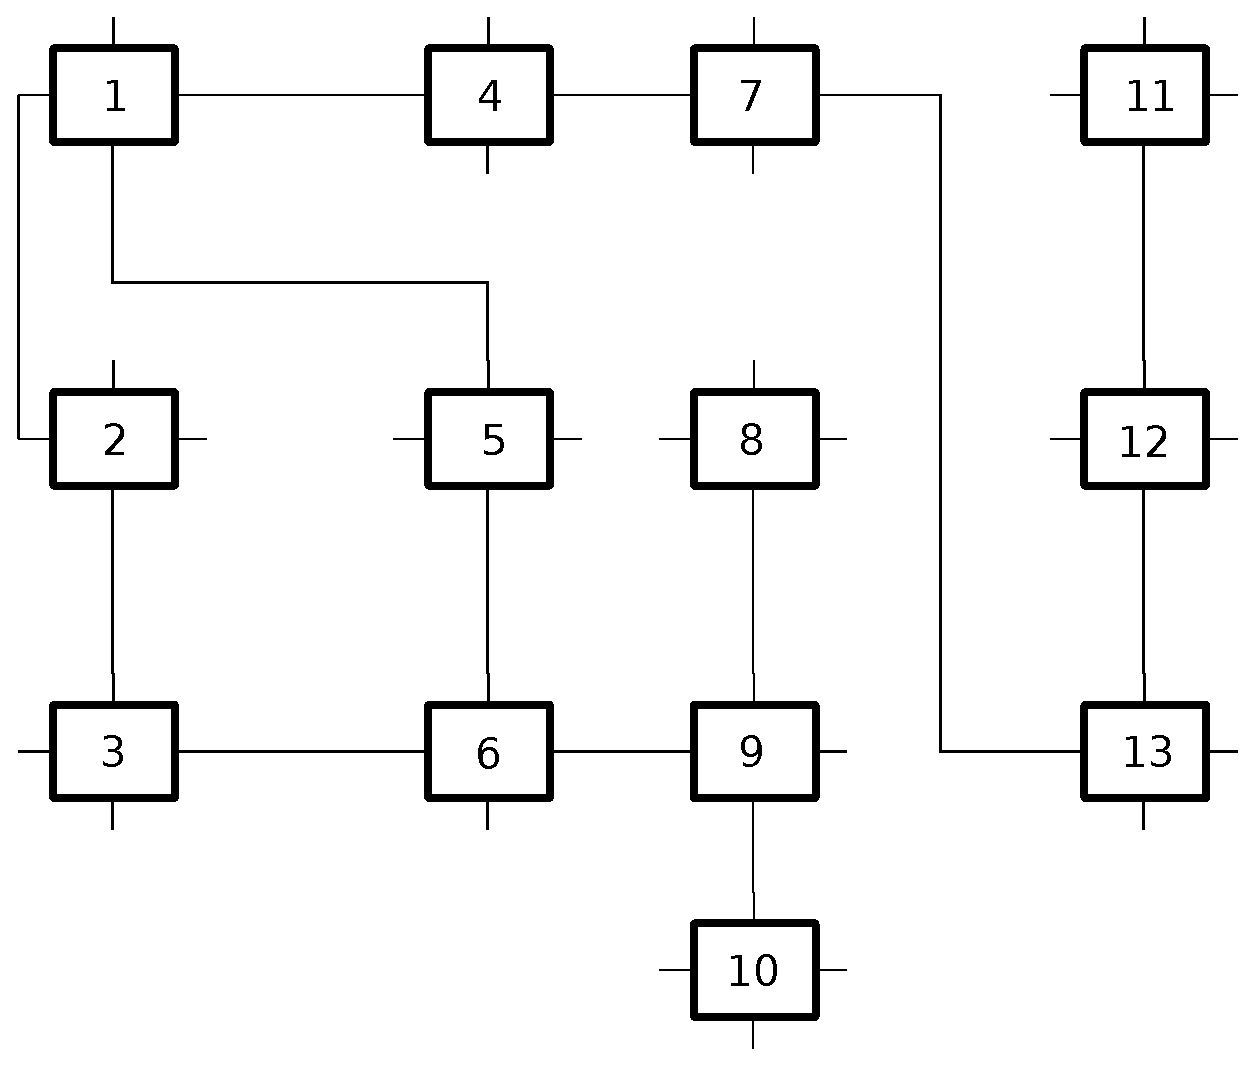
\includegraphics[width=0.3\textwidth]{../Figures_and_tables/Figure4_NativeTopolgy}
\caption{Native topology}
\label{nativeFig}
\end{figure}

This simple topology has the lowest communication cost theoretically possible, since $h_{i,j} = 1$ for all edges $e_{i,j}$. Hence, this sets a benchmark for the minimum communication cost. Any topology that includes this as a subgraph will have the same communication cost. Hence, this topology is intended to be the basis for the algorithm~\ref{poorestAlgo}. When this technique is applied to the input graph in fig.~\ref{inputFig}, the resultant topology is illustrated in  fig.~\ref{nativeFig}.
\section{Poorest Neighbour Algorithm}
The native topology has the lowest possible communication cost, as mentioned in section~\ref{nativeSection}. However, it might not be link fault tolerant. To achieve that, we add some more links. But, we still include the entire native topology so as to keep communication cost to the minimum. In the following algorithm, we test whether each link $l_{i,j}$ in the native topology has an alternate path connecting routers $r_i$ and $r_j$ (going in the descending order of the corresponding weights $w_{i,j}$). If not, we connect it to a neighbouring router with the lowest degree (defined in section~\ref{degree}). The rationale behind this algorithm is that the edges with highest weights should have the lowest possible hops in order to reduce the total communication cost and that the routers should have similar loads (and therefore similar degrees). This is the 'poorest neighbour' algorithm (algorithm~\ref{poorestAlgo}).
\begin{algorithm}
\caption{Poorest Neighbour Algorithm}\label{poorestAlgo}
\begin{algorithmic}[1]
\renewcommand{\algorithmicrequire}{\textbf{Input:}}
\renewcommand{\algorithmicensure}{\textbf{Output:}}
\newcommand{\algorithmicbreak}{\textbf{break}}
\newcommand{\BREAK}{\STATE \algorithmicbreak}
\newcommand{\algorithmiccontinue}{\textbf{continue}}
\newcommand{\CONTINUE}{\STATE \algorithmiccontinue}
\newcommand{\letvariable}{\textbf{let }}
\newcommand{\FUNCTION}{\textbf{function }}
 \REQUIRE CFG $G(N,E)$
 \ENSURE  TG $T(R,L)$
 \STATE Generate the native topology $T(R,L)$ using algorithm~\ref{nativeAlgo}.
 \FORALL {links $l_{i,j}$ in $L$}
 \IF {there exists an alternate path between $r_i$ and $r_j$}
 \CONTINUE
 \ELSE
 \STATE \letvariable $r_l$ be the router with the lower degree from routers $r_i$ and $r_j$
 \STATE \letvariable $r_h$ be the router with the higher degree from routers $r_i$ and $r_j$
 \STATE from the list of all the neighbouring routers of $r_h$, \\
 \letvariable $r_p$ be the router with the lowest degree. \COMMENT {$r_p$ is the `poorest' neighbour of $r_h$.}
 \STATE create link $l_{p,h}$ connecting routers $r_p$ and $r_h$.
 \STATE add $l_{p,h}$ to $L$ in $T(R,L)$.
 \ENDIF
 \ENDFOR \label{insertHere}
% \STATE execute \FUNCTION validate($T(R,L)$) \COMMENT{explained in section~\ref{} and defined in~\ref{}}
\RETURN $T(R,L)$
\end{algorithmic}
\end{algorithm}
When this algorithm is applied to the CFG in fig.~\ref{inputFig}, result looks like fig.~\ref{poorestFig}.
\begin{figure}
\centering
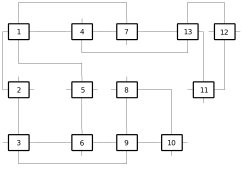
\includegraphics[width=0.4\textwidth]{../Figures_and_tables/Figure5_PoorestNeighbor}
\caption{Result of poorest neighbour algorithm}
\label{poorestFig}
\end{figure}
\section{De-Bruijn's Algorithm}
De Bruijn's graph is a popular algorithm which is widely used in the field of Bioinformatics%citation needed
. Works such as \cite{b7} suggest De Bruijn's graph as an alternate topology and compared its energy consumption with popular regular topologies like Mesh and Torus. This graph is inherently link fault tolerant and has lower energy consumption than regular topologies like Mesh as established by \cite{b7}. It may also contain more than one alternate path for a pair of nodes. The algorithm~\ref{deBruijnAlgo} is also explained in \cite{b9}. In the later sections of the paper, its performance is compared against the poorest neighbour algorithm (algorithm~\ref{poorestAlgo}).
\begin{algorithm}
\caption{De-Bruijn's Algorithm}\label{deBruijnAlgo}
\begin{algorithmic}[1]
\renewcommand{\algorithmicrequire}{\textbf{Input:}}
\renewcommand{\algorithmicensure}{\textbf{Output:}}
\newcommand{\algorithmicbreak}{\textbf{break}}
\newcommand{\BREAK}{\STATE \algorithmicbreak}
\newcommand{\algorithmiccontinue}{\textbf{continue}}
\newcommand{\CONTINUE}{\STATE \algorithmiccontinue}
\newcommand{\letvariable}{\textbf{let }}
\newcommand{\FUNCTION}{\textbf{function }}
 \REQUIRE CFG $G(N,E)$
 \ENSURE  TG $T(R,L)$
\STATE \letvariable $R = N$ \COMMENT{the number of routers in TG and cores in CFG is the same since there is a one to one mapping}
\STATE Connect routers $r_1$ and $r_2$ with link $l_{1,2}$ and add it to $L$ in $TG(R,L)$.
\STATE \letvariable $p = 2$ and $c = p + 1 = 3$.
\WHILE{$c < R$}
\STATE Connect routers $r_c$ and $r_p$ with link $l_{c,p}$ and add it to $L$ in $TG(R,L)$.
\STATE $c = c + 1$.
\IF{$c$ is odd}
\STATE $p = p +1$.
\ENDIF
\ENDWHILE
\STATE \letvariable $p = R$ and $c = p - 1$.
\STATE \letvariable $e = N \mod 2$
\WHILE{$c > 0$}
\STATE Connect routers $r_c$ and $r_p$ with link $l_{c,p}$ and add it to $L$ in $TG(R,L)$.
\STATE $c = c - 1$.
\IF{$c \mod 2 = e$}
\STATE $p = p - 1$.
\ENDIF
\ENDWHILE
\RETURN $T(R,L)$
\end{algorithmic}
\end{algorithm}
When applied to the CFG in fig.~\ref{inputFig}, the result looks like fig.~\ref{deBruijnFig}
\begin{figure}
\centering
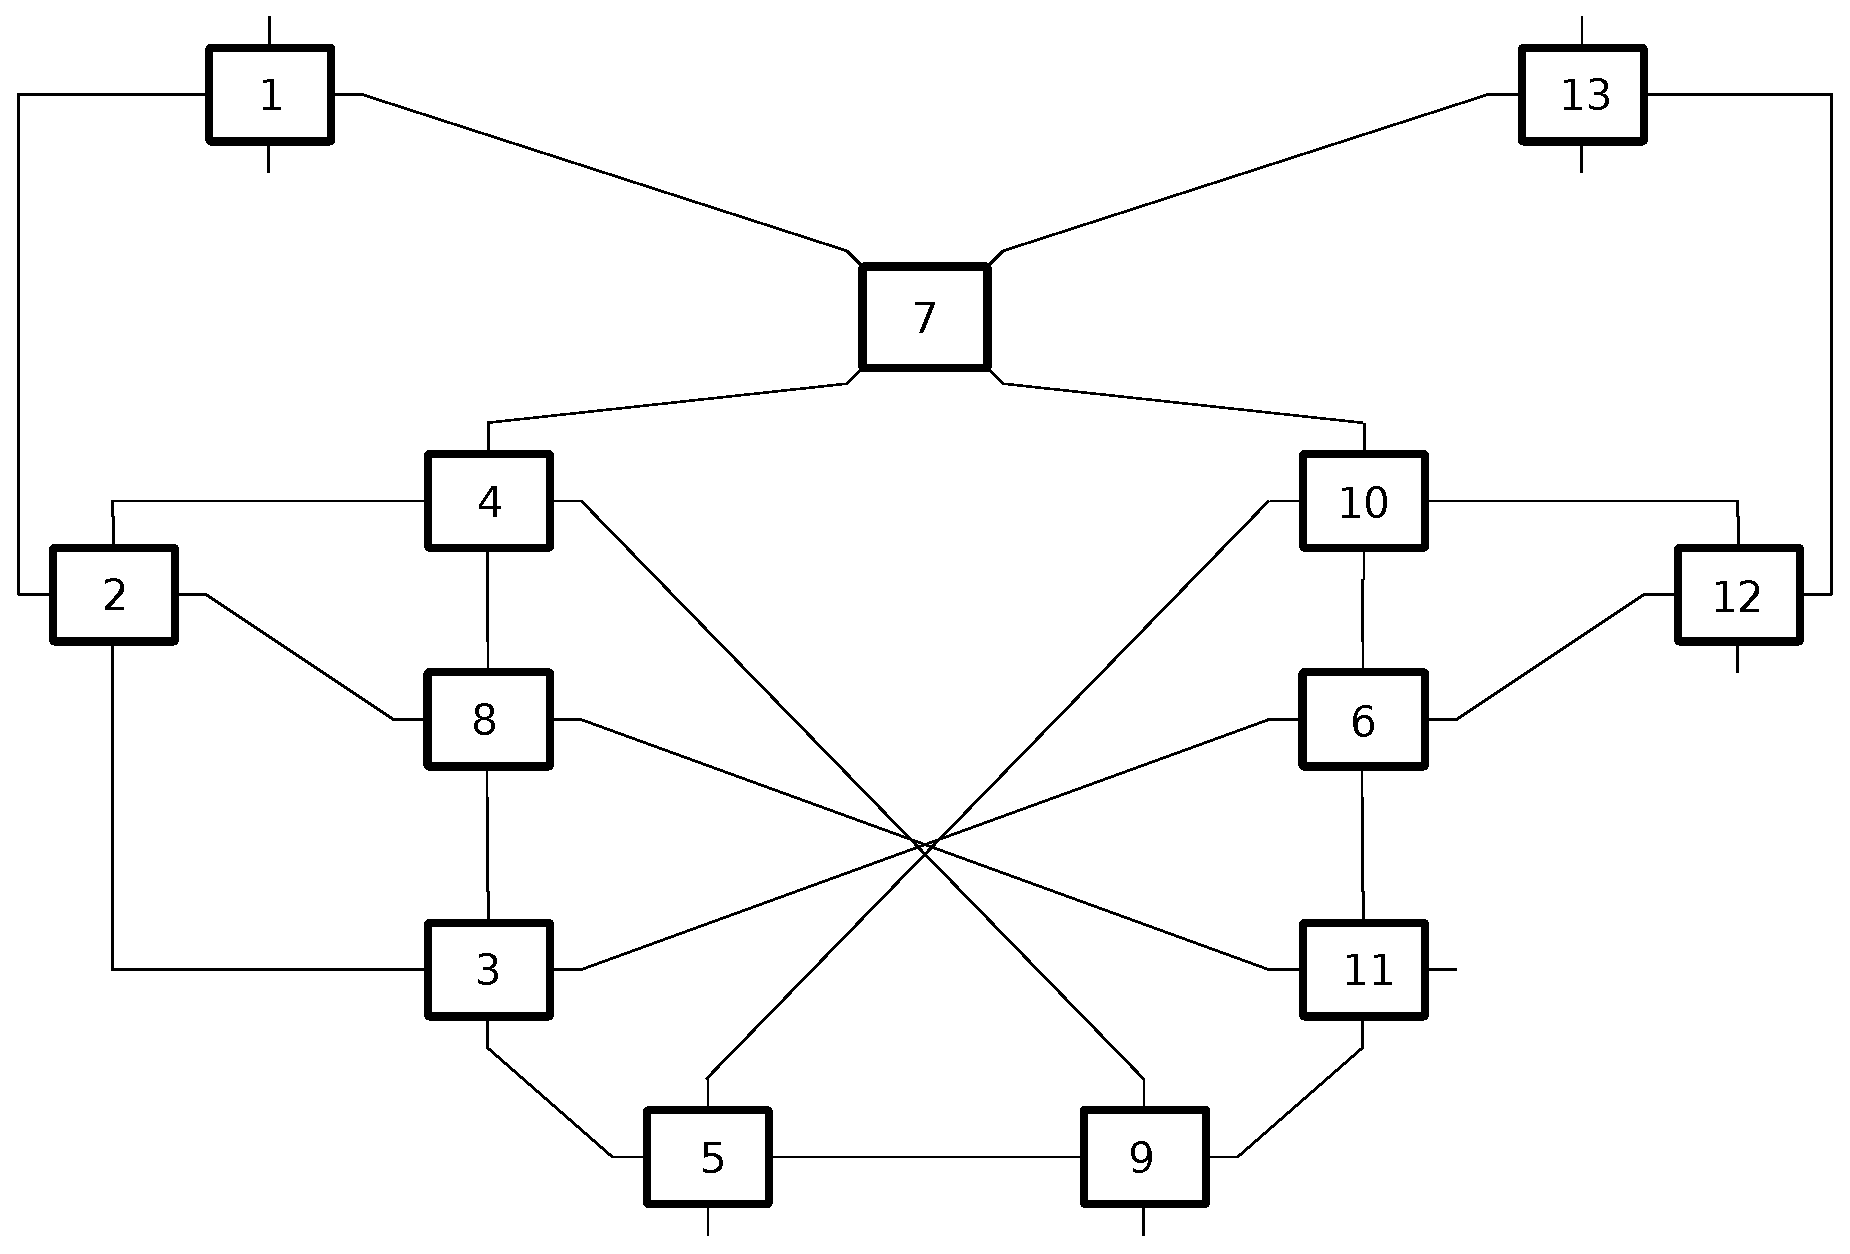
\includegraphics[width=0.45\textwidth]{../Figures_and_tables/Figure6_DeBruijn}
\caption{De Bruijn's graph}
\label{deBruijnFig}
\end{figure}
\section{Observations}
The main objective of this paper is to create a topology with 100\% link fault tolerance. However, as seen in table~\ref{faultTolerance}, the poorest neighbour algorithm does not always provide 100\% link fault tolerance. We investigate the cause and find a solution for this problem in this section. With the solution proposed here, the poorest neighbour algorithm provides 100\% link fault tolerance in all tested cases.
\begin{table}[htbp]
\caption{Link fault tolerance}
\begin{center}
\begin{tabular}{|c|c|c|c|}
\hline
\textbf{Number}&\multicolumn{3}{|c|}{\textbf{Link fault tolerance}} \\
\cline{2-4} 
\textbf{of} & \textbf{\textit{Poorest neighbour}}& \textbf{\textit{Poorest neighbour}}& \textbf{\textit{De}} \\
\textbf{cores} & \textbf{\textit{(without}}& \textbf{\textit{(with solution)}}& \textbf{\textit{Bruijn's}} \\
\textbf{} & \textbf{\textit{solution)}}& \textbf{\textit{}}& \textbf{\textit{graph}} \\
\hline
8& 100& 100& 100 \\
\hline
24& 100& 100& 100\\
\hline
30& 86.20& 100& 100\\
\hline
64& 100& 100& 100\\
\hline
64& 99.0& 100& 100\\
\hline
128& 100& 100& 100\\
\hline
\end{tabular}
\label{faultTolerance}
\end{center}
\end{table}
\subsection{Fail Case: Isolated Pair}
Consider a disconnected graph like the one shown in fig.~\ref{isolatedPairFig}. The poorest neighbour algorithm first checks if each link has an alternate path for connecting the two end routers of that link. If yes, then it does nothing. If no, then the algorithm seeks to connect one of the routers with a neighbour of the other router. But in this graph, consider the routers $r_7$ and $r_8$. None of these routers have another neighbour to connect to. No connection is thus made, and the resulting topology does not provide 100\% link fault tolerance.
\begin{figure}
\centering
\includegraphics[width=0.3\textwidth]{../Figures_and_tables/Figure7_IsolatedPair}
\caption{Graph with an isolated pair}
\label{isolatedPairFig}
\end{figure}
\subsection{Proposed solutions}\label{solution}
In this case, the proposed solution is to modify the algorithm to connect the routers to the router (in the rest of the topology) with the lowest degree. Here, the routers $r_1$ and $r_6$ are of degree 2. Thus, if we choose router $r_6$, the resulting topology would look something like fig.~\ref{isolatedPairSolutionFig}. Similarly, if we choose router $r_1$, the links would be established between $r_7$, $r_8$ and $r_1$. This procedure is illustrated in algorithm~\ref{isolatedSolutionAlgo} and is to be performed after the completion of poorest neighbour algorithm (\ref{poorestAlgo}).
\begin{algorithm}
\caption{Solution to isolated pair scenario}\label{isolatedSolutionAlgo}
\begin{algorithmic}[1]
\renewcommand{\algorithmicrequire}{\textbf{Input:}}
\renewcommand{\algorithmicensure}{\textbf{Output:}}
\newcommand{\algorithmicbreak}{\textbf{break}}
\newcommand{\BREAK}{\STATE \algorithmicbreak}
\newcommand{\algorithmiccontinue}{\textbf{continue}}
\newcommand{\CONTINUE}{\STATE \algorithmiccontinue}
\newcommand{\letvariable}{\textbf{let }}
\newcommand{\FUNCTION}{\textbf{function }}
\REQUIRE TG $T(R,L)$
\ENSURE  TG $T(R,L)$
\FORALL{$l_{i,j}$ such that $degree(r_i) = 1$ and $degree(r_j) = 1$}
\STATE from the rest of the topology, find $r_p$ with lowest degree. \COMMENT{if there are more than one routers with the lowest degree, choose one arbitrarily.}
\STATE connect both routers $r_i$ and $r_j$ to $r_p$.
\ENDFOR
\RETURN $T(R,L)$
\end{algorithmic}
\end{algorithm}
\begin{figure}
\centering
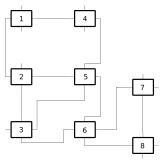
\includegraphics[width=0.25\textwidth]{../Figures_and_tables/Figure8_IsolatedPairSolution}
\caption{proposed solution}
\label{isolatedPairSolutionFig}
\end{figure}
\section{Results}
In this section, the comparison is performed for all the topology generation methods. The mentioned algorithms were implemented in JAVA and simulated by generating different networks used in the paper. Every algorithm was evaluated by considering overall communication cost and the required number of links. The results are available in\cite{d1}. The binaries of implementations and input data are available in\cite{d2}. Table~\ref{commCostTable} compares the communication cost of the topologies generated by native, poorest neighbour and De Bruijn's algorithms against the number of cores in the input CFG. It is clear from this comparison that the communication cost of the topology generated by poorest neighbour always matches the communication cost of the native topology irrespective of the number of cores contained in the CFG. Hence, poorest neighbour algorithm is highly scalable for fault tolerant topology generation. Also, we can infer that for a given input graph, the communication cost of the topology generated by poorest neighbour is very less compared to the topology generated by De Bruijn's algorithm. Thus, DeBruijn's algorithm is not very scalable in comparison. 
	Table~\ref{numberOfLinksTable} compares the number of links required for the topologies generated by the poorest neighbour and De Bruijn's algorithms. Lesser the number of links, lower the hardware cost. In this aspect, the poorest neighbour algorithm is marginally better than De Bruijn's algorithm.
\begin{table}[htbp]
\caption{Communication cost}
\begin{center}
\begin{tabular}{|c|c|c|c|}
\hline
\textbf{Number}&\multicolumn{3}{|c|}{\textbf{Communication cost}} \\
\cline{2-4} 
\textbf{of cores} & \textbf{\textit{Native}}& \textbf{\textit{Poorest neighbour}}& \textbf{\textit{De Bruijn's graph}} \\
\hline
8& 576& 576& 704 \\
\hline
24& 131& 131& 401\\
\hline
30& 88& 88& 364\\
\hline
64& 24,608& 24,608& 423,165\\
\hline
64& 6,063& 6,063& 93,454\\
\hline
128& 55,404& 55,404& 1,777,704\\
\hline
128& 11,963& 11,963& 380,437\\
\hline
128& 26,281& 26,281& 892,604\\
\hline
128& 163,837& 163,837& 5,437,165\\
\hline
128& 137,777& 137,777& 4,667,287\\
\hline
\end{tabular}
\label{commCostTable}
\end{center}
\end{table}

\begin{table}[htbp]
\caption{Number of links}
\begin{center}
\begin{tabular}{|c|c|c|c|}
\hline
\textbf{Number}&\multicolumn{3}{|c|}{\textbf{Number of links}} \\
\cline{2-4} 
\textbf{of cores} & \textbf{\textit{Native}}& \textbf{\textit{Poorest neighbour}}& \textbf{\textit{De Bruijn's graph}} \\
\hline
8& 8& 9& 13 \\
\hline
24& 21& 33& 44\\
\hline
30& 24& 37& 56\\
\hline
64& 95& 108& 125\\
\hline
64& 59& 103& 125\\
\hline
128& 207& 234& 253\\
\hline
128& 127& 211& 253\\
\hline
128& 180& 202& 253\\
\hline
128& 236& 265& 253\\
\hline
128& 192& 229& 253\\
\hline
\end{tabular}
\label{numberOfLinksTable}
\end{center}
\end{table}
\section{Conclusion}
The native topology set the benchmark for communication cost. Both De Bruijn's and poorest neighbour algorithms (with the additional procedure mentioned in section~\ref{solution}) provide 100\% link fault tolerance in all the tested scenarios. However, the latter outperforms the former with significantly lower communication cost as well as marginally lower hardware costs.
\begin{thebibliography}{00}
\bibitem{b1} Benini, L., Micheli, G. D. ``Network on chips: a new SoC paradigm," IEEE Computer, Vol. 35, No. 1, pp.70-78, 2002. 
\bibitem{b2} Fathollah Karimi Koupaei, Ahmad Khademzadeh, Majid Janidarmian, ``Fault tolerant application specific network-on-chip," Proceedings of the World Congress on Engineering and Computer Science 2011, Vol II, WCECS 2011, October 2011
\bibitem{b3}  Suleyman Tosun, Vahid B. Ajabshir, Ozge Mercanoglu, and Ozcan Ozturk, ``Fault tolerant topology generation method for application specific network-on-chips," IEEE Transactions On Computer - Aided Design Of Integrated Circuits And Systems, vol. 34, no. 9, September 2015
\bibitem{b8} G. Ascia, V. Catania, M. Palesi, ``Multi-objective mapping for mesh-based NoC architectures," in: ODES SSS 2004. International Conference in Hardware/ Software Codesign and System Synthesis, 8-10 Sept. 2004,  p. 182-187.
\bibitem{b9} Sharma, Tharesh. ``Fault Tolerant Network on chips Topologies." Reliable Networks-On-Chip in the Many Core Era. Universit�t Stuttgart - SS09, Stuttgart. July 7, 2009. Seminar Report, p. 14 - 17.
\bibitem{b4} Hosseinzadeh, F., Bagherzadeh, N., Khademzadeh, A., Janidarmianm, M. (2014) ``Fault tolerant optimization for application specific network-on-chip architecture," LNEE, Vol. 247, No. 2014, pp. 363-381
\bibitem{b5} Koupaei, F. K., Khademzadeh, A., Janidarmian, M. (2011)  ``fault-tolerant application-specific network-on-chip," In Proceedings of the World Congress on Engineering and Computer Science.
\bibitem{b10} Becker M., Kr�mker M., Szczerbicka H. (2015) ``Evaluating Heuristic Optimization, Bio-Inspired and Graph-Theoretic Algorithms for the Generation of Fault-Tolerant Graphs with Minimal Costs,''. In: Kim K. (eds) Information Science and Applications. Lecture Notes in Electrical Engineering, vol 339. Springer, Berlin, Heidelberg, pp 1033-1041
\bibitem{b6} Yesil, S., Tosun S., Ozturk, O. (2016) ``FPGA implementation of a fault-tolerant application-specific NoC design,"�2016 International Conference on Design and Technology of Integrated Systems in Nanoscale Era (DTIS), Istanbul, pp. 1-6.
\bibitem{b7} M. Hosseinabady, M. R. Kakoee, J. Mathew and D. K. Pradhan, ``Reliable network-on-chip based on generalized de Bruijn graph," 2007 IEEE International High Level Design Validation and Test Workshop, Irvine, CA, 2007, pp. 3-10.
\bibitem{b11} Pengfei Yang, Quan Wang, Wei Li, Zhibin Yu, Hongwei Ye, ``A Fault Tolerance NoC Topology and Adaptive Routing Algorithm,'' 2016 13th International Conference on Embedded Software and Systems (ICESS), pp. 42-47
\bibitem{d1} Shah, Parth; Kanniganti, Abhishek (2017): Simulation results. figshare. 
https://doi.org/10.6084/m9.figshare.5590015.v2. 
Retrieved: 07:47, Nov 12, 2017 (GMT)
\bibitem{d2} Shah, Parth; Kanniganti, Abhishek (2017): PoorestNeighbourAlgorithm. figshare.
https://doi.org/10.6084/m9.figshare.5593468.v1
Retrieved: 10:10, Nov 12, 2017 (GMT)
\end{thebibliography}

\end{document}
